\section{Constitutive model for uncycled exogenously crosslinked tissue}
\subsection{Constitutive model for exogenous crosslinking}

	We have previously developed the first constitutive model for exogenously crosslinked collagenous tissues \cite{sacks_novel_2016} and determined the following three contributors to the mechanical response: collagen fibers, exogenously crosslinked matrix and fiber-fiber interactions. 
	In particular, we found the fiber ensemble interaction term to be especially important in modeling exogenously crosslinked tissues, accounting for approximately 30\% of the stress in the fully loaded state (Fig. \ref{fig:EXLforms}A). 
	To determine the model form of the interaction component, we used the remaining stress after subtracting the collagen fiber response and exogenously crosslinked matrix response from the mechanical response of the tissue after exogenous crosslinking (Fig. \ref{fig:EXLforms}A). 
	In that study, we consider three possible forms of interactions: intra-fiber \textbf{ensemble} (Fig. \ref{fig:EXLforms}B) (an ensemble being a family of fiber sharing a common orientation), ensemble-ensemble rotations, and ensemble-ensemble relative extensions (Fig. \ref{fig:EXLforms}C\&D). 
	We found that intra-fiber ensemble and ensemble-ensemble rotations were not consistent with the experimental data, whereas ensemble-ensemble extensional interactions were able to explain all of the remaining stress. 
	
	We developed the fiber ensemble interaction model form utilizing the pseudo invariant $I_8$, and separated it into its rotational and extensional components\cite{sacks_novel_2016},
\begin{equation}
\begin{gathered}
I_8 = \mathbf{n}_0\left( \alpha\right)\cdot\mathbf{C}\cdot\mathbf{n}_0\left( \beta\right) = \lambda_\alpha \lambda_\beta \cos(\alpha - \beta), \\
I_8^{\mathrm{ext}} = \lambda_\alpha \lambda_\beta, \qquad I_8^{\mathrm{rot}} = \cos(\alpha - \beta) = \frac{I_8}{\lambda_\alpha \lambda_\beta},
\end{gathered}
\end{equation}
where $\mathbf{n}_0$ is an unit vector pointing along $\theta$, $I_8^{ext}$ is the pseudo invariant for ensemble-ensemble relative extensions, and $I_8^{rot}$ is the ensemble-ensemble rotations. 
From this, we established model form for the interactions to be
\begin{equation}
\Psi_{\mathrm{int}} = \frac{d_0}{4}\int\displaylimits_\alpha \int\displaylimits_\beta \Gamma\left(\alpha\right)\Gamma \left( \beta \right)\left[ e^{d_1(\lambda_\alpha \lambda_\beta - 1)^2}-1 \right] \mathrm{d}\alpha\, \mathrm{d}\beta,
\end{equation}
where $\Gamma$ is the fiber orientation distribution (ODF), and $d_0$ and $d_1$ are material constants. 
	However, this model form is still essentially phenomenological. 
	Specifically, while it is sufficient to model the mechanical response in the range of the acquired experimental data, we have no method for predicting how it will change with changes in dimensions with cyclic loading. Thus, an extension to this model component is necessary.

\begin{figure}[hbt]
\centering
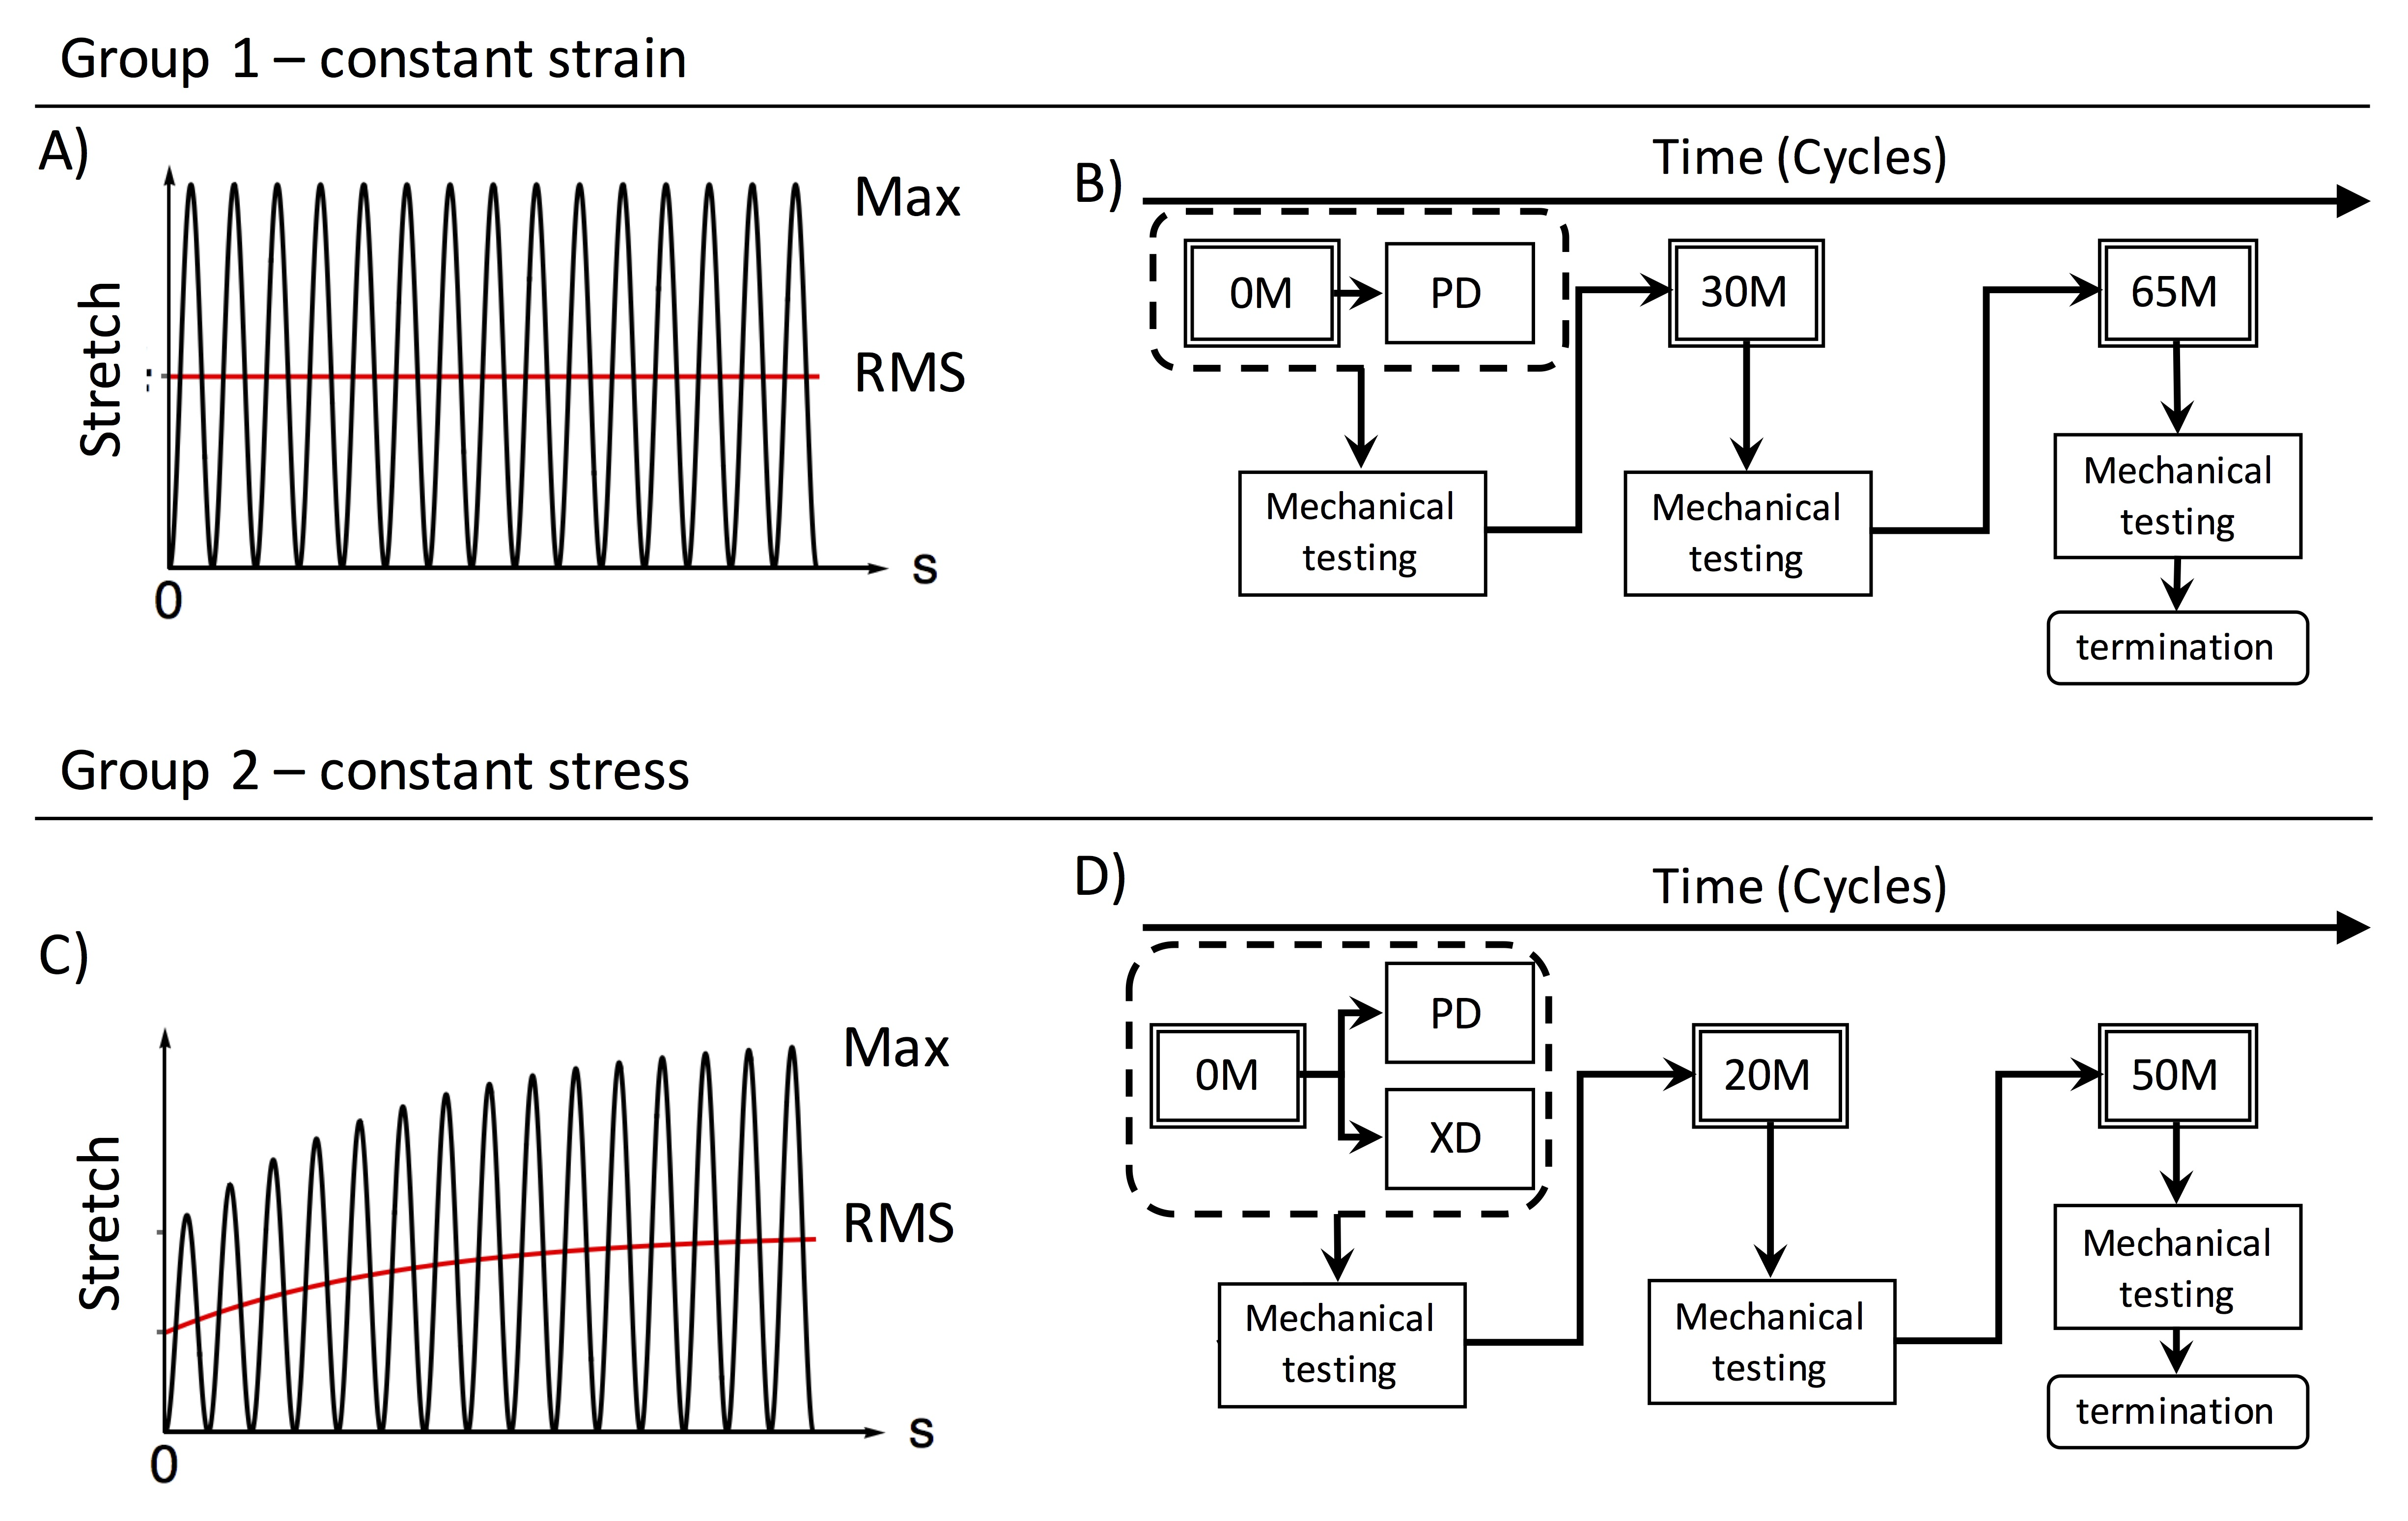
\includegraphics[width=0.5\paperwidth]{Images/chapter4/figure5}
\caption{A) The mechanical response of exogenously crosslinked BP, which is composed of 3 parts: (C)ollagen(Red), (M)atrix(Blue), and the fiber ensemble (I)nteractions (Green). B) Illustration for intra-ensemble interactions due to crosslinking is shown. C) Ensemble-ensemble interactions could be separated into rotational effects and extensional effects. }
\label{fig:EXLforms}
\end{figure}

\subsection{Extension of the structural derivation of the fiber-fiber interactions term}

The key to our approach in the constitutive model for the permanent set effect is to use the change in the collagen fiber architecture to predict the new mechanical response. 
Thus, having a full structural model, including a full structural derivation of the fiber-fiber interactions, is crucial. 
As in the previous model form \cite{sacks_novel_2016}, we will only keep the extensional component $I_8^{ext}$. In addition, since collagen fibers do not bear stress until fully straightened \cite{soares_biomechanical_2016}, we also assume that \emph{collagen fibers do not play a role in the interactions of the fiber ensembles until they are straightened}. Given the true fiber stretch ($\lambda_t$) as defined in Zhang et al. \cite{zhang_meso_2016}, $\lambda_t = \lambda_{ens}/\lambda_s$, we incorporated the collagen slack stretch, $\lambda_s$, into the invariant, with
\begin{equation}
I_8^{\mathrm{ext}} = \frac{\lambda_\alpha \lambda_\beta}{\lambda^\alpha_s \lambda_s^\beta}.
\end{equation}
To develop the form for the interactions, we start from the strain energy. 
At the ensemble level, we integrate over the slack stretch $(D)$, as define in Zhang \textit{et al.} \cite{zhang_meso_2016}, of fiber ensembles orienting along $\alpha$ and $\beta$, 
\begin{equation}
\Psi_{\mathrm{int}}^{\mathrm{ens}} = \frac{\eta_I}{2} \int\displaylimits_1^{\lambda_\alpha} \int\displaylimits_1^{\lambda_\beta} D\left( x_\alpha \right) D\left( x_\beta \right) \left( \frac{\lambda_\alpha \lambda_\beta}{x_\alpha x_\beta} - 1\right)^2 \,\mathrm{d}x_\alpha \,\mathrm{d}x_\beta.
\end{equation}
This is then integrated over the fiber ODF, $\Gamma$, for the tissue-level model
\begin{equation}
\Psi_{\mathrm{int}} = \frac{\eta_I}{2} \int\displaylimits_\alpha \int\displaylimits_\beta \Gamma(\alpha) \Gamma(\beta) \int\displaylimits_1^{\lambda_\alpha} \int\displaylimits_1^{\lambda_\beta} D\left( x_\alpha \right) D\left( x_\beta \right) \left( \frac{\lambda_\alpha \lambda_\beta}{x_\alpha x_\beta} - 1\right)^2 \,\mathrm{d}x_\alpha \,\mathrm{d}x_\beta \,\mathrm{d}\alpha \,\mathrm{d}\beta.
\end{equation}
The second Piola Kirchhoff stress, using $\mathbf{S}=2\frac{\partial\Psi}{\partial\mathbf{C}}$, is 
\begin{equation} \label{eq:interaction}
\begin{split}
\mathbf{S}_{\mathrm{int}} = \phi_C \eta_I \int\displaylimits_\alpha \int\displaylimits_\beta \Gamma \left(\alpha \right) \Gamma \left( \beta \right) 
\left[ \left\lbrace 
\int\displaylimits_1^{\lambda_\alpha} \int\displaylimits_1^{\lambda_\beta} 
\frac{2 \lambda_\beta D(x_\alpha) D(x_\beta)}{x_\alpha x_\beta} 
\left( \frac{\lambda_\alpha}{x_\alpha} \frac{\lambda_\beta}{x_\beta} - 1\right) \mathrm{d}x_\alpha \, \mathrm{d}x_\beta \right.\right. +&\\
\left. \left. \int\displaylimits_1^{\lambda_\beta} D(x_\beta) \left( \frac{\lambda_\beta}{x_\beta} -1  \right)^2 \mathrm{d}x_\beta \right\rbrace \right.  \frac{\mathbf{n}_\alpha \otimes \mathbf{n}_\alpha}{\lambda_\alpha} +& \\
\left. \left\lbrace
\int\displaylimits_1^{\lambda_\alpha} \int\displaylimits_1^{\lambda_\alpha} 
\frac{2 \lambda_\beta D(x_\alpha) D(x_\beta)}{x_\alpha x_\beta} 
\left( \frac{\lambda_\alpha}{x_\alpha} \frac{\lambda_\beta}{x_\beta} - 1\right) \mathrm{d}x_\alpha \, \mathrm{d}x_\beta 
\right. \right. +&\\
\left. \left. \int\displaylimits_1^{\lambda_\alpha} D(x_\alpha) \left( \frac{\lambda_\alpha}{x_\alpha} -1  \right)^2 \mathrm{d}x_\alpha \right\rbrace \frac{\mathbf{n}_\beta \otimes \mathbf{n}_\beta}{\lambda_\beta}  \right]& \mathrm{d}\alpha \, \mathrm{d}\beta.
\end{split}
\end{equation}
This model form has only one constant $\eta_I$ to account for all interactions. The remaining mechanisms are all structurally based, which is determined through a convection of the collagen fiber architecture. 
